\documentclass[11pt,spanish,a4paper]{article}
% Versión 1.er cuat 2021 Víctor Bettachini < bettachini@df.uba.ar >

% Versión 1.er cuat 2021 Víctor Bettachini < bettachini@df.uba.ar >

\usepackage[T1]{fontenc}
\usepackage[utf8]{inputenc}

\usepackage[spanish, es-tabla]{babel}
\def\spanishoptions{argentina} % Was macht dass?
% \usepackage{babelbib}
% \selectbiblanguage{spanish}
% \addto\shorthandsspanish{\spanishdeactivate{~<>}}

\usepackage{graphicx}
\graphicspath{{./figuras/}}
% \usepackage{float}

\usepackage[arrowdel]{physics}
\newcommand{\pvec}[1]{\vec{#1}\mkern2mu\vphantom{#1}}
% \usepackage{units}
\usepackage[separate-uncertainty=true, multi-part-units=single, locale=FR]{siunitx}
\usepackage{isotope} % $\isotope[A][Z]{X}\to\isotope[A-4][Z-2]{Y}+\isotope[4][2]{\alpha}

\usepackage{tasks}
\usepackage[inline]{enumitem}
% \usepackage{enumerate}

\usepackage{hyperref}

% \usepackage{amsmath}
% \usepackage{amstext}
\usepackage{amssymb}

\usepackage{tikz}
\usepackage{tikz-dimline}
\usetikzlibrary{math}
\usetikzlibrary{arrows.meta}
% \usetikzlibrary{snakes}
% \usetikzlibrary{calc}
\usetikzlibrary{decorations.pathmorphing}
\usetikzlibrary{patterns}

\usepackage[hmargin=1cm,vmargin=1.6cm,nohead]{geometry}
% \voffset-3.5cm
% \hoffset-3cm
% \setlength{\textwidth}{17.5cm}
% \setlength{\textheight}{27cm}

\usepackage{lastpage}
\usepackage{fancyhdr}
\pagestyle{fancyplain}
\fancyhead{}
\fancyfoot{{\tiny \textcopyright DF, FCEyN, UBA}}
\fancyfoot[C]{ {\tiny Actualizado al \today} }
\fancyfoot[RO, LE]{Pág. \thepage/\pageref{LastPage}}
\renewcommand{\headrulewidth}{0pt}
\renewcommand{\footrulewidth}{0pt}


\begin{document}
\begin{center}
	\textbf{Física 2} (Físicos) \hfill \textcopyright {\tt DF, FCEyN, UBA}\\
	\textsc{\LARGE Rayos y frentes de onda}
\end{center}

Los ejercicios con (*) entrañan una dificultad adicional. Son para investigar después de resolver los demás.


\begin{enumerate}


\section*{Interfaz entre medios}

\item 
\begin{enumerate}
	\item (*) Demuestre que la función: $\Psi (\vec{r}, t) = A \operatorname{e}^{ i (\vec{k} \cdot \vec{r} \pm \omega t) }$, con $\vec{k} = k_x \hat{x} + k_y \hat{y} + k_z \hat{z}$ un vector constante y $\vec{r}= x \hat{x} + y \hat{y} + z \hat{z}$, es solución de la ecuación de ondas tridimensional.
	Sugerencia: exprese el Laplaciano en coordenadas cartesianas.
	\item Analice el significado físico de $\Psi (\vec{r}, t)$.
	¿Cómo son los frentes de onda?
	¿Cuál es la relación entre el vector $\vec{k}$ y los frentes de onda?
	¿Hacia dónde se desplazan los frentes de onda al transcurrir $t$?
	¿A qué velocidad?
\end{enumerate}


\item (*)
\begin{minipage}[t][2cm]{0.75\textwidth}
Una onda de presión \( \delta p_i (\vec{r},t)\) incide desde el aire describiendo un ángulo $\theta$ con la normal a una superficie de agua calma.
Si usamos notación compleja la describimos como $\delta p_{i} (\vec{r}, t) = A_i \operatorname{e}^{i (\vec{k}_{i} \cdot \vec{r} - \omega t) }$, siendo $\vec{k}_i = \frac{ \omega }{ v_s } \left( \sen(\theta) \hat{x} + \cos(\theta) \hat{y} \right)$.
Hallar las ondas reflejadas y transmitidas, $\delta p_r (\vec{r}, t) = A_r \operatorname{e}^{ i ( \vec{k}_r \cdot \vec{r} - \omega t) }$ y $\delta p_t (\vec{r}, t) = A_t \operatorname{e}^{ i (\vec{k}_t \cdot \vec{r} - \omega t) }$.
\end{minipage}
\begin{minipage}[c][0.4cm][t]{0.2\textwidth}
	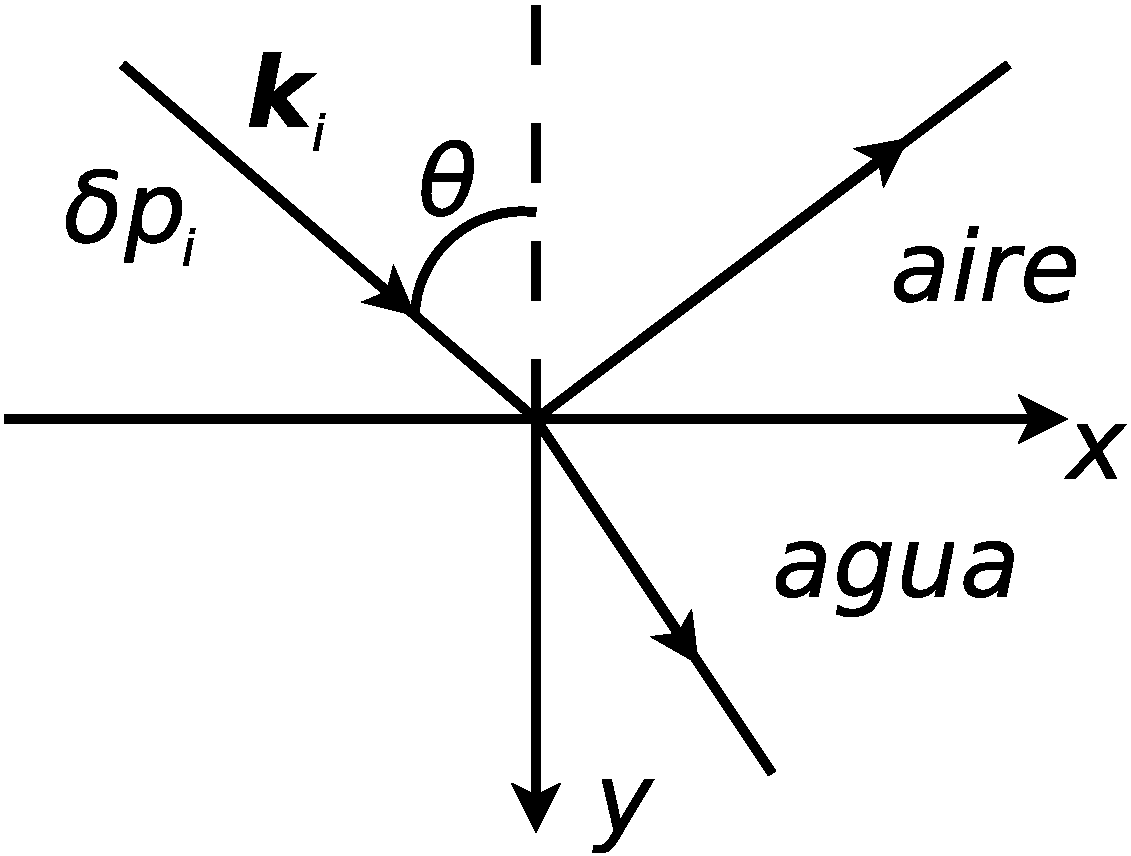
\includegraphics[width=\textwidth]{ej2-13}
\end{minipage}


\section*{Fermat | Ibn Sahl - Snell}

\item
A partir del principio de Fermat deducir la ley de Ibn Sahl - Snell para la refracción de la luz entre dos medios de índices $n_1$ y $n_2$, separados por una superficie plana.


\item
\begin{enumerate}
	\item (*) Si un rayo parte del punto $A=(0,1,0)$, se refleja en el espejo plano $(x,0,z)$ y pasa por el punto $B=(4,3,0)$, averigüe en qué punto sobre el plano del espejo se refleja y los ángulos de incidencia y reflexión.
	Aplicar Fermat e interpretar físicamente las soluciones. 
	\item (*) Un rayo directo entre $A$ y $B$ recorre un menor camino óptico que el hallado en (a), ¿es esto contradictorio?
\end{enumerate}



%\item (*) Un espejo elíptico de focos $A$ y $B$, tiene el primero una fuente puntual.
%Los espejos esférico y plano dibujados son tangentes al elíptico en $C$.
%Sabiendo que el camino óptico de un rayo que sale de $A$, se refleja en $C$ y luego pasa por $B$, es estacionario en la elipse, obtenga cualitativamente si el camino óptico es máximo, mínimo o estacionario cuando se refleja en cada uno de los espejos.


\section*{Espejos planos}

\item (*) Demuestre que la imagen dada por un espejo plano de una fuente puntual es, sin ninguna aproximación, otra fuente puntual, ubicada simétricamente respecto del plano del espejo.
Analice los casos que corresponden a objetos reales o virtuales.


\item ¿Cuál es la mínima longitud de un espejo plano vertical para que un hombre de \SI{1.8}{\metre} se vea entero?
¿Es importante conocer la distancia hombre-espejo? 


\item (*)
\begin{minipage}[t][1.5cm]{0.8\textwidth}
Realice un diagrama de rayos que le permita localizar las imágenes de la flecha que se muestra en la figura.
Para un punto de la flecha dibuje una porción del frente de ondas emergente y los correspondientes frentes reflejados.
\end{minipage}
\begin{minipage}[c][0.6cm][t]{0.1\textwidth}
	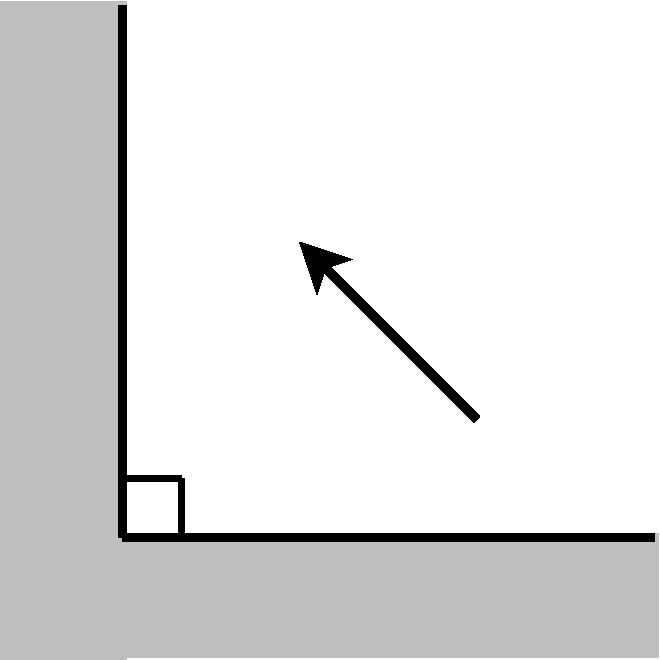
\includegraphics[width=\textwidth]{ej3-11}
\end{minipage}



\item
\begin{minipage}[t][0cm]{0.65\textwidth}
Dos espejos planos forman un ángulo $\alpha$ como lo indica la figura.
\end{minipage}
\begin{minipage}[c][1.5cm][t]{0.3\textwidth}
	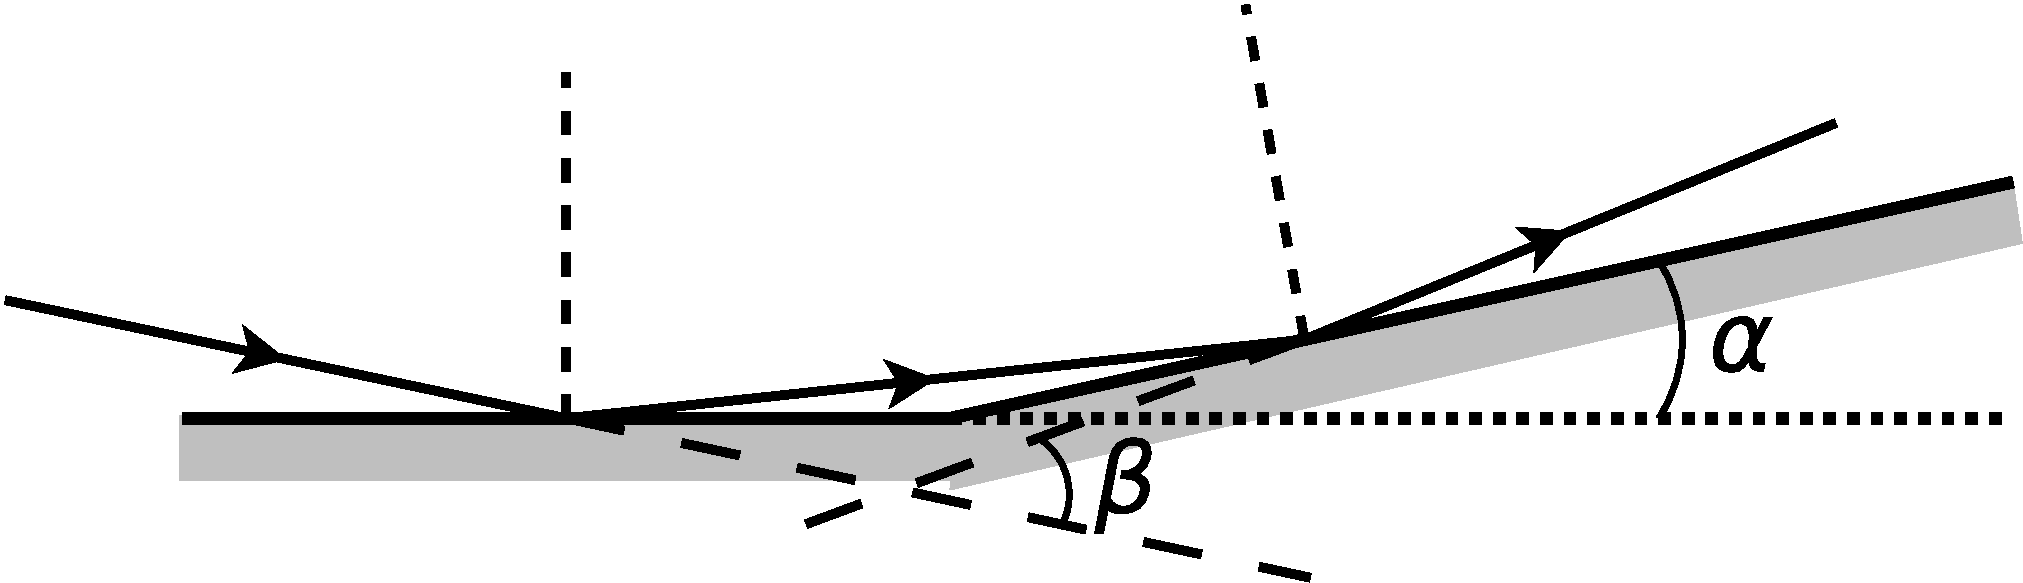
\includegraphics[width=\textwidth]{ej3-12}
\end{minipage}
\begin{enumerate}
	\item Un rayo de luz contenido en un plano perpendicular a la intersección de los espejos incide sobre uno de ellos, se refleja e incide en el otro (ver figura).
	Calcule el ángulo \(\beta\) que forman los rayos incidente y emergente.
	\item (*) Suponga la misma geometría que en a) pero ahora iluminada por una fuente puntual, demuestre que las imágenes se encuentran sobre una circunferencia con centro en el vértice de los espejos.
	En el caso en que la fuente está ubicada de tal modo que sólo se producen dos imágenes, y que el ángulo es muy pequeño, calcule la distancia entre ellas (espejos de Fresnel).
\end{enumerate}


% \section*{Espejos curvos}

\item
\begin{enumerate}
	\item (*) Partiendo de la ecuación de las dioptras obtenga la ecuación de los espejos esféricos. 
	\item ¿Cómo se modifica la distancia focal de un espejo esférico si se lo sumerge en agua?
	\item Un espejo esférico cóncavo produce una imagen cuyo tamaño es el doble del tamaño del objeto, siendo la distancia objeto--imagen de \SI{15}{\centi\metre}.
	Calcule la distancia focal del espejo.
\end{enumerate}



\item (*) Una esfera maciza de radio $R$ e índice de refracción \num{1.5} ha sido espejada en una mitad de su superficie.
Se coloca un objeto sobre el eje de la esfera a distancia $2R$ del vértice de la semiesfera no espejada.
Hallar:
\begin{enumerate}
\item La imagen final, en forma analítica, luego de todas las refracciones
y reflexiones que hayan tenido lugar.
\item El aumento y las características de la imagen final.
\item Ídem (a) mediante trazado de rayos.
\end{enumerate}
 % mejor con diotra


\end{enumerate}

\end{document}
